%----- Ben:

%- Baselinecuts (vor baseline vergleichen mit nach baseline) + Leptonveto

%- Stackedergebnis plot - Susy gefunden? Spoiler: Nein (Zwishcnergebnis)
\begin{frame}
	\frametitle{A first Glance at Data}
	Before analysis the data pre-selection cuts are taken to reduce the amount of data and improve the calculation time of the MC simulation. 
	\begin{block}{Pre-Selection Cuts}
		\begin{itemize}
			\item  $H_T > 300\si{GeV}$ and $N_{\si{jets}} \geq 2$
			\item  $\slashed{H}_T > 100\si{GeV}$ in case of QCD
		\end{itemize}
	\end{block}
	
	\begin{center}
		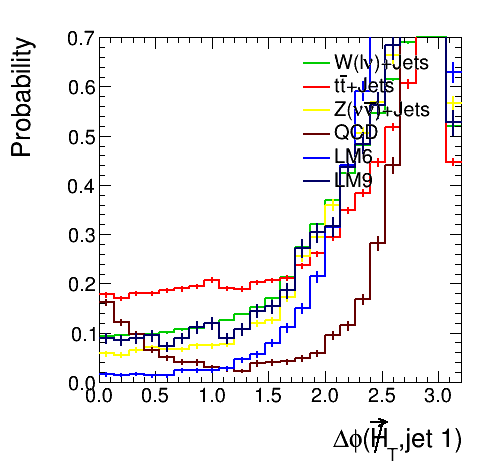
\includegraphics[width = 0.4\textwidth]{plots10/hDeltaPhi1.png}
		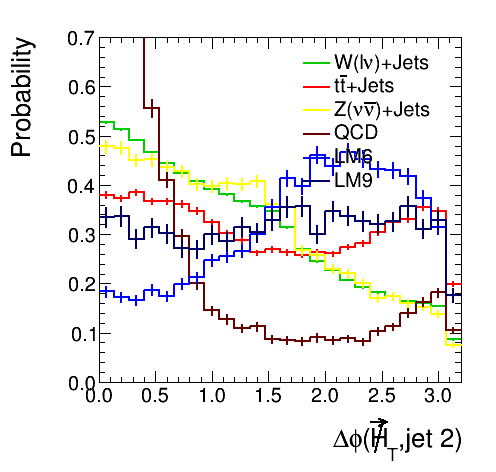
\includegraphics[width = 0.4\textwidth]{plots10/hDeltaPhi2.png}
	\end{center}

\end{frame}

 
\begin{frame}
	\frametitle{Baseline-Cuts}
	\begin{block}{My Title}
		\begin{itemize}
			\item no lepton events with  $p_T > 50 \si{ GeV}$ and $\lvert\eta\rvert < 2.5$ are considered
			\item $N_{\si{jets}} > 3$ with $p_T > 50 \si{ GeV}$ and $\lvert\eta\rvert < 2.4$
			\item $H_T > 500\si{GeV}$ with $p_T > 50 \si{ GeV}$ and $\lvert\eta\rvert < 2.5$
			\item $\slashed{H}_T > 200\si{GeV}$ with $p_T > 30 \si{GeV}$ and $\lvert\eta\rvert < 5.0$	
			\item $\Delta\phi(\si{jet}_{1,2},\slashed{H}_T) > 0.5$ and  $\Delta\phi(\si{jet}_3,\slashed{H}_T) > 0.3$
		\end{itemize}
	\end{block}
	
		\begin{center}
		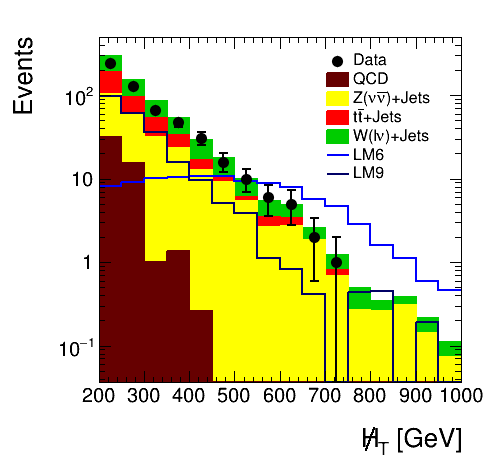
\includegraphics[width = 0.4\textwidth]{plots10/hDataVsMC_Mht.png}
		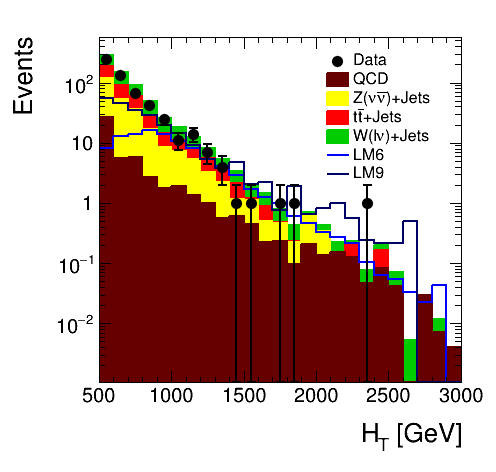
\includegraphics[width = 0.4\textwidth]{plots10/hDataVsMC_Ht.png}
	\end{center}
\end{frame}


\begin{frame}
	\frametitle{Results after applying baseline cuts}
	\begin{block}{background understanding}
		\begin{itemize}
			\item improved understanding and characterization of background 
			\item QCD-Events are well filtered
			\item no evidence for SUSY-Particles so far
		\end{itemize}
	\end{block}
	
	\begin{center}
		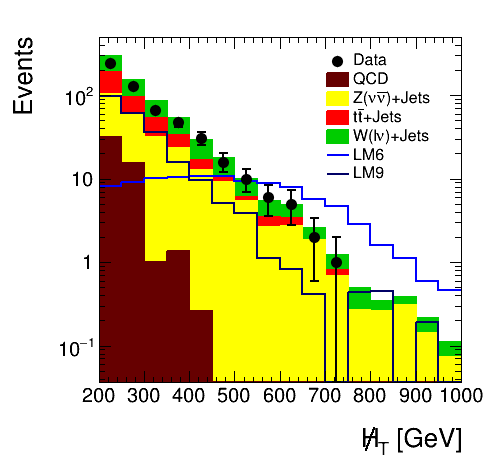
\includegraphics[width = 0.4\textwidth]{plots10/hDataVsMC_Mht.png}
		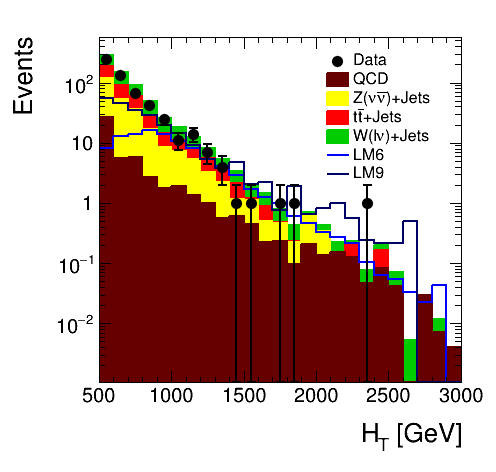
\includegraphics[width = 0.4\textwidth]{plots10/hDataVsMC_Ht.png}
	\end{center}

\end{frame}